\section{External Interface Requirements}
\label{sec:external_interface_requirements}%

\subsection{User Interfaces}
\label{subsec:user_interfaces}%
The eMALL’s user interfaces are a website and a mobile application;
the first is developed to be used mainly by CPOs with a dedicated login section for businesses but can be used by EVDs too.
The mobile application is available for Android and iOS and provides an enhanced experience as compared to the website
since it offers users personalized suggestions based on their location.
The website and the app should be easy to use since they will be used mostly by middle-aged users,
who might not always be familiar with the technology.
A “quick booking” section dedicated to facilitating the booking process might be included,
for those EVDs who are used to booking a charge at the same charging station (based on suggestions given by AI).

\subsection{Hardware Interfaces}
\label{subsec:hardware_interfaces}%
The system only requires a smartphone or computer with an internet connection and web browser to access websites or mobile applications.
Furthermore, eMALL communicates with the EV through its company's API to get the current battery level, the charging state,
so if it is plugged in and if it is charging, and the number of routable kilometers obtained on the current battery level.
To access personalized suggestions, based on EV’s position, the device in use has to be able to detect its location with a GPS or Glonass localization system.
%TODO: think id there is something you can write in this subsection

\subsection{Software Interfaces}
\label{subsec:software_interfaces}%

\subsection{Communication Interfaces}
\label{subsec:communication_interfaces}%
The eMALL system needs to communicate with other actors to offer functionalities to the users;
the communication is bidirectional and permits eMALL to obtain the desired data and serve elaborated data.
Below are listed different communication interfaces used to exchange information with users:
\begin{itemize}
    \item \textbf{CPMS and Charging Points.} The CPMSs offered to the CPO communicate with the charging point
    through the OCPP communication protocol.
    Thanks to it, the system can manage the charging session, given the possibility of starting and stopping it.
    Another significant functionality offered by OCPP is the diagnostic of the charging point:
    a CPO can reboot its charging spots, can get their log, and can update their firmware.
    %TODO: Does it make sense to put an example of an external system
    \item \textbf{eMALL and EVs.} The eMALL system communicates with the EVs registered by the EVD\@.
    As explained in the domain assumption section, we suppose that there is a third-party system that offers its API
    so to get the status of the battery of the EV. %An example of a system that provides these features is Smartcar,
    %which is already used by companies like AmpUp or BeCharge to remotely retrieve the battery level and remaining range of the EVs.
    \item \textbf{CPMS and DSOs.} The CPMSs offered to the CPO communicate with the DSOs through their APIs.
    CPOs can get selling prices set by the DSOs and they can decide from which DSO to acquire electricity.
    \item \textbf{eMALL and third-party payment services.} The \verb|eMALL| system offers the possibility to pay through
    external payment services to the EVD. The communication happens thanks to APIs offered by the companies that handle payments.
\end{itemize}


\section{Functional Requirements}
\label{sec:functional_requirements}%

\subsection{Requirements}
\label{subsec: requirements}%

%TODO: complete the table after having completed the use cases
\newcounter{req}
\setcounter{req}{1}
\newcommand{\creq}{\thereq\stepcounter{req}}
\begin{center}
    \begin{longtable}{|l|l|}
        \hline
        \textbf{ID} & \textbf{Description} \\
        \hline
        R\creq      &                      \\
        \hline
        \caption{Requirements.}
        \label{tab: req}%
    \end{longtable}
\end{center}

\subsection{Mapping on goals}
\label{subsec: map_on_g}%

%TODO: complete the table after having done the requirements
\newcounter{mg}
\setcounter{mg}{1}
\newcommand{\cmg}{\themg\stepcounter{mg}}
\begin{center}
    \begin{longtable}{|l|l|l|}
        \hline
        \textbf{Goal} & \textbf{Domain assumptions} & \textbf{Requirements} \\
        \hline
        G\cmg         &                             &                       \\
        \hline
        G\cmg         &                             &                       \\
        \hline
        G\cmg         &                             &                       \\
        \hline
        G\cmg         &                             &                       \\
        \hline
        G\cmg         &                             &                       \\
        \hline
        G\cmg         &                             &                       \\
        \hline
        G\cmg         &                             &                       \\
        \hline
        G\cmg         &                             &                       \\
        \hline
        G\cmg         &                             &                       \\
        \hline
        G\cmg         &                             &                       \\
        \hline
        G\cmg         &                             &                       \\
        \hline
        G\cmg         &                             &                       \\
        \hline
        \caption{Mapping on goals.}
        \label{tab: map_on_g}%
    \end{longtable}
\end{center}
%TODO: correct the diagrams if you add or remove use cases

\subsection{Use case diagrams}
\label{subsec: use_case_diag}%

\textbf{Unregistered EVD}
\begin{figure} [H]
    \begin{center}
        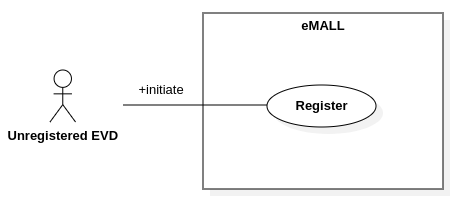
\includegraphics[width=0.9\linewidth]{Images/UseCaseDiagrams/unregistered_EVD_use_case_diagram}
        \caption{Unregistered EVD use case diagram}
        \label{fig: unreg_EVD_diag}
    \end{center}
\end{figure}

\textbf{Registered EVD}
\begin{figure} [H]
    \begin{center}
        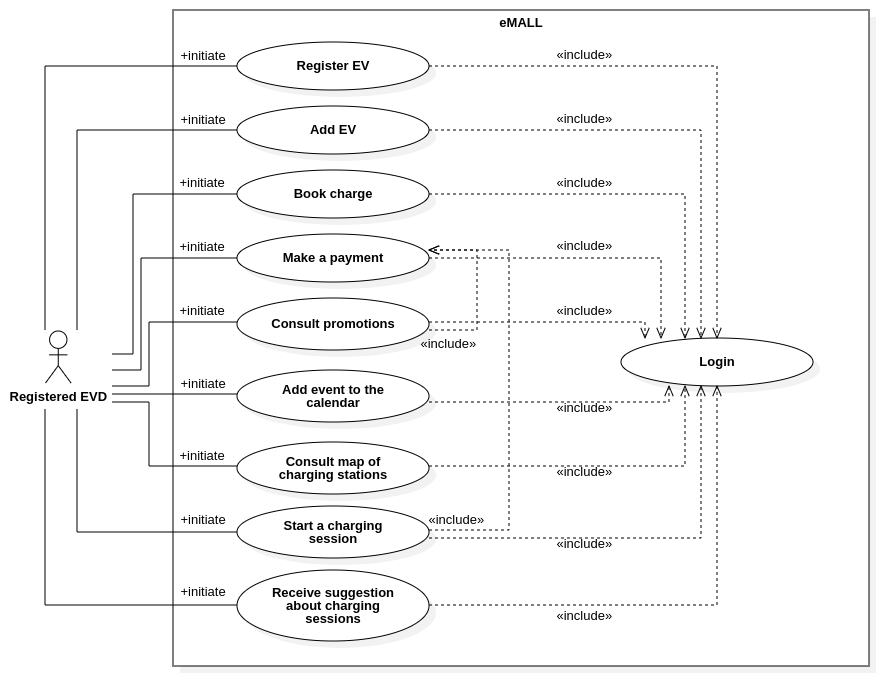
\includegraphics[width=0.9\linewidth]{Images/UseCaseDiagrams/registered_EVD_use_case_diagram}
        \caption{Unregistered EVD use case diagram}
        \label{fig: reg_EVD_diag}
    \end{center}
\end{figure}

\textbf{CPO}
\begin{figure} [H]
    \begin{center}
        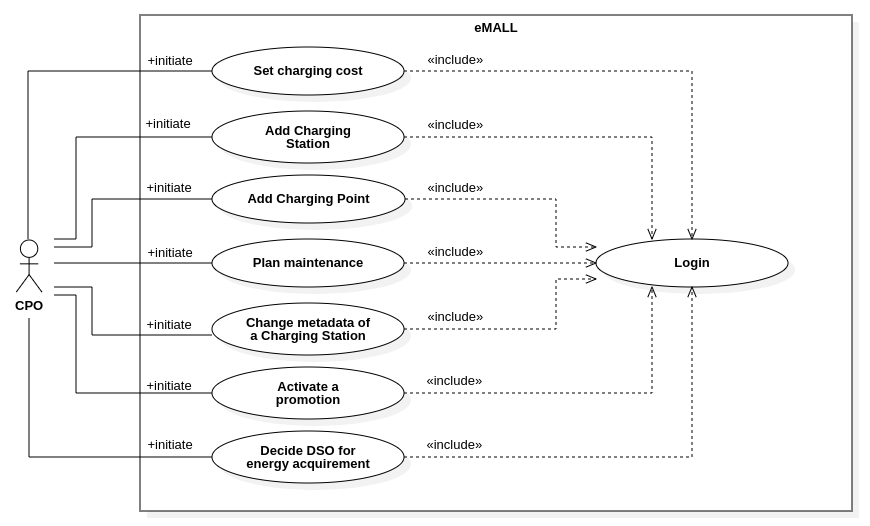
\includegraphics[width=0.9\linewidth]{Images/UseCaseDiagrams/CPO_use_case_diagram}
        \caption{Unregistered EVD use case diagram}
        \label{fig: cpo_diag}
    \end{center}
\end{figure}

\subsection{Use cases}
\label{subsec: use_cases}%
%TODO: write it better
In this section, they are explained and represented the main identified use cases.
There is a table with entry conditions, event flow, exit conditions and exception for each of them, and a sequence diagram
that shows the messages exchanged between the entities and the called functions.

\subsection{Mapping on requirements}
\label{subsec: map_on_req}%
\newcounter{mr}
\setcounter{mr}{1}
\newcommand{\cmr}{\themr\stepcounter{mr}}
\begin{center}
    \begin{longtable}{|l|l|}
        \hline
        \textbf{Use Case} & \textbf{Requirements} \\
        \hline
        \caption{Mapping on requirements.}
        \label{tab: map_on_req}
    \end{longtable}
\end{center}


\section{Performance Requirements}
\label{sec:performance_requirements}%
\textbf{Number of users.} \\
According to a market analysis conducted by \verb|MOTUS-E| in September 2022,
the number of fully electric vehicles and plug-in hybrid vehicles registered in Italy is 320.776.
If we suppose that the eMALL system will be used by one in every three EVDs,
the system should guarantee that it can handle an overall of 100.000 clients. \\
So, we can consider that the system should be able to handle th $50\%$ of them could be connected simultaneously. \\
\\
\textbf{Data storage} \\
From the data storage point of view, the \verb|eMALL| system should consider several sources of data:
\begin{itemize}
    \item \textbf{EVD's personal data.} We consider that $5\ KB$ is enough for the storage of personal information of an EVD\@.
    Considering $10^5$ EVDs, the system needs:
    \begin{center}
        $10^5\cdot5\ KB = 488,3\ MB$
    \end{center}
    \item \textbf{EVD's calendar.} One of the functionalities offered by the \verb|eMALL| system is to insert new activities
    into EVD's calendar.
    The events have not much information: they specify starting time and destination of the activity.
    We can assume that each event requires $1 KB$ of storage.
    Considering all the potential users and assuming that they insert three activities a day, for the first year the system needs:
    \begin{center}
        $10^5\cdot 3\cdot 365\cdot 1\ KB = 104,43\ GB$
    \end{center}
    \item \textbf{History of charging sessions.} The \verb|eMALL| system should save the information of all the charging sessions.
    We assume that the information of each charging session requires $3\ KB$ of storage.
    To decide how many times we want to assume a generic EVD charges his EV, we have to consider different factors,
    such as the EVDs' habits, the storage of their EV's battery, and the distances they can drive during the day.
    For example, an EVD who drives long distances every day and whose EV has a small battery may need to charge
    it more frequently than an EVD with a larger battery who only drives short distances.
    Similarly, an EVD that can access fast charging infrastructure may be able to charge his EV less frequently than
    a driver who only has access to slower charging stations.
    So, it is reasonable to assume that a generic EVD charges his EV twice a week. \\
    For the first year, the system needs:
    \begin{center}
        $10^5\cdot \frac{365}{7} \cdot 2\cdot 3\ KB = 29,84\ GB$
    \end{center}
    \item \textbf{CPO's personal data.} If we consider that in Italy there could be more or less 50 CPOs,
    as we did for the EVDs, we can assume that one in every three CPOs subscribes to the \verb|eMALL| system.
    We consider enough $5\ KB$ of storage for each profile.
    So, the system needs:
    \begin{center}
        $20\cdot 5\ KB = 100\ KB$
    \end{center}
    \item \textbf{Charging points registration.} Each CPO registers information about their charging points distributed in the territory.
    Referring again to the market analysis conducted by \verb|MOTUS-E|, in September 2022,
    there were a total of 32.776 charging points in Italy.
    So, we can assume that all the CPOs register 11.000 charging points all together.
    We consider enough $5\ KB$ of storage for the registration of each charging spot.
    So, the system needs:
    \begin{center}
        $11 000\cdot 5\ KB = 53,71\ MB$
    \end{center}
\end{itemize}
The rest of storage needed is about the several functionalities offered to the EVDs and to the CPOs.
So, after summing all the values obtained in the previous list, we overestimate the memory suggested for the first year
of life of the system.
Summing all the values, it is:
\begin{center}
    $488,3\ MB + 104,43\ GB + 29,84\ GB + 100\ KB + 53,71\ MB = 134,8\ GB$
\end{center}
So, a memory storage of $200\ GB$ will be enough for the first year of the \verb|eMALL| system. \\
\\
\textbf{Time response} \\
The \verb|eMALL| system should handle all the requests within 3 seconds, given that there are not strict time response requirements.



\section{Design Constraints}
\label{sec:design_constraints}%

\subsection{Standards compliance}
\label{subsec:standards_compliance}%

\subsection{Hardware limitations}
\label{subsec:hardware_limitations}%

\subsection{Any other constraint}
\label{subsec:any_other_constraint}%


\section{Software System Attributes}
\label{sec:software_system_attributes}%

\subsection{Reliability}
\label{subsec:reliability}%

\subsection{Availability}
\label{subsec:availability}%

\subsection{Security}
\label{subsec:security}%

\subsection{Maintainability}
\label{subsec:maintainability}%

\subsection{Portability}
\label{subsec:portability}%
